\documentclass{article}

\usepackage{graphicx}
\usepackage{tikz}
\usepackage{tikzsymbols}
\usetikzlibrary{calc,patterns,shapes.geometric}
\pagestyle{empty}
\usepackage[margin=0pt]{geometry}
\geometry{papersize={14in,12in}}

\def\centerarc[#1](#2)(#3:#4:#5){\draw[#1] ($(#2)+({#5*cos(#3)},{#5*sin(#3)})$) arc (#3:#4:#5);}

\begin{document}
	\begin{figure}
		\centering
		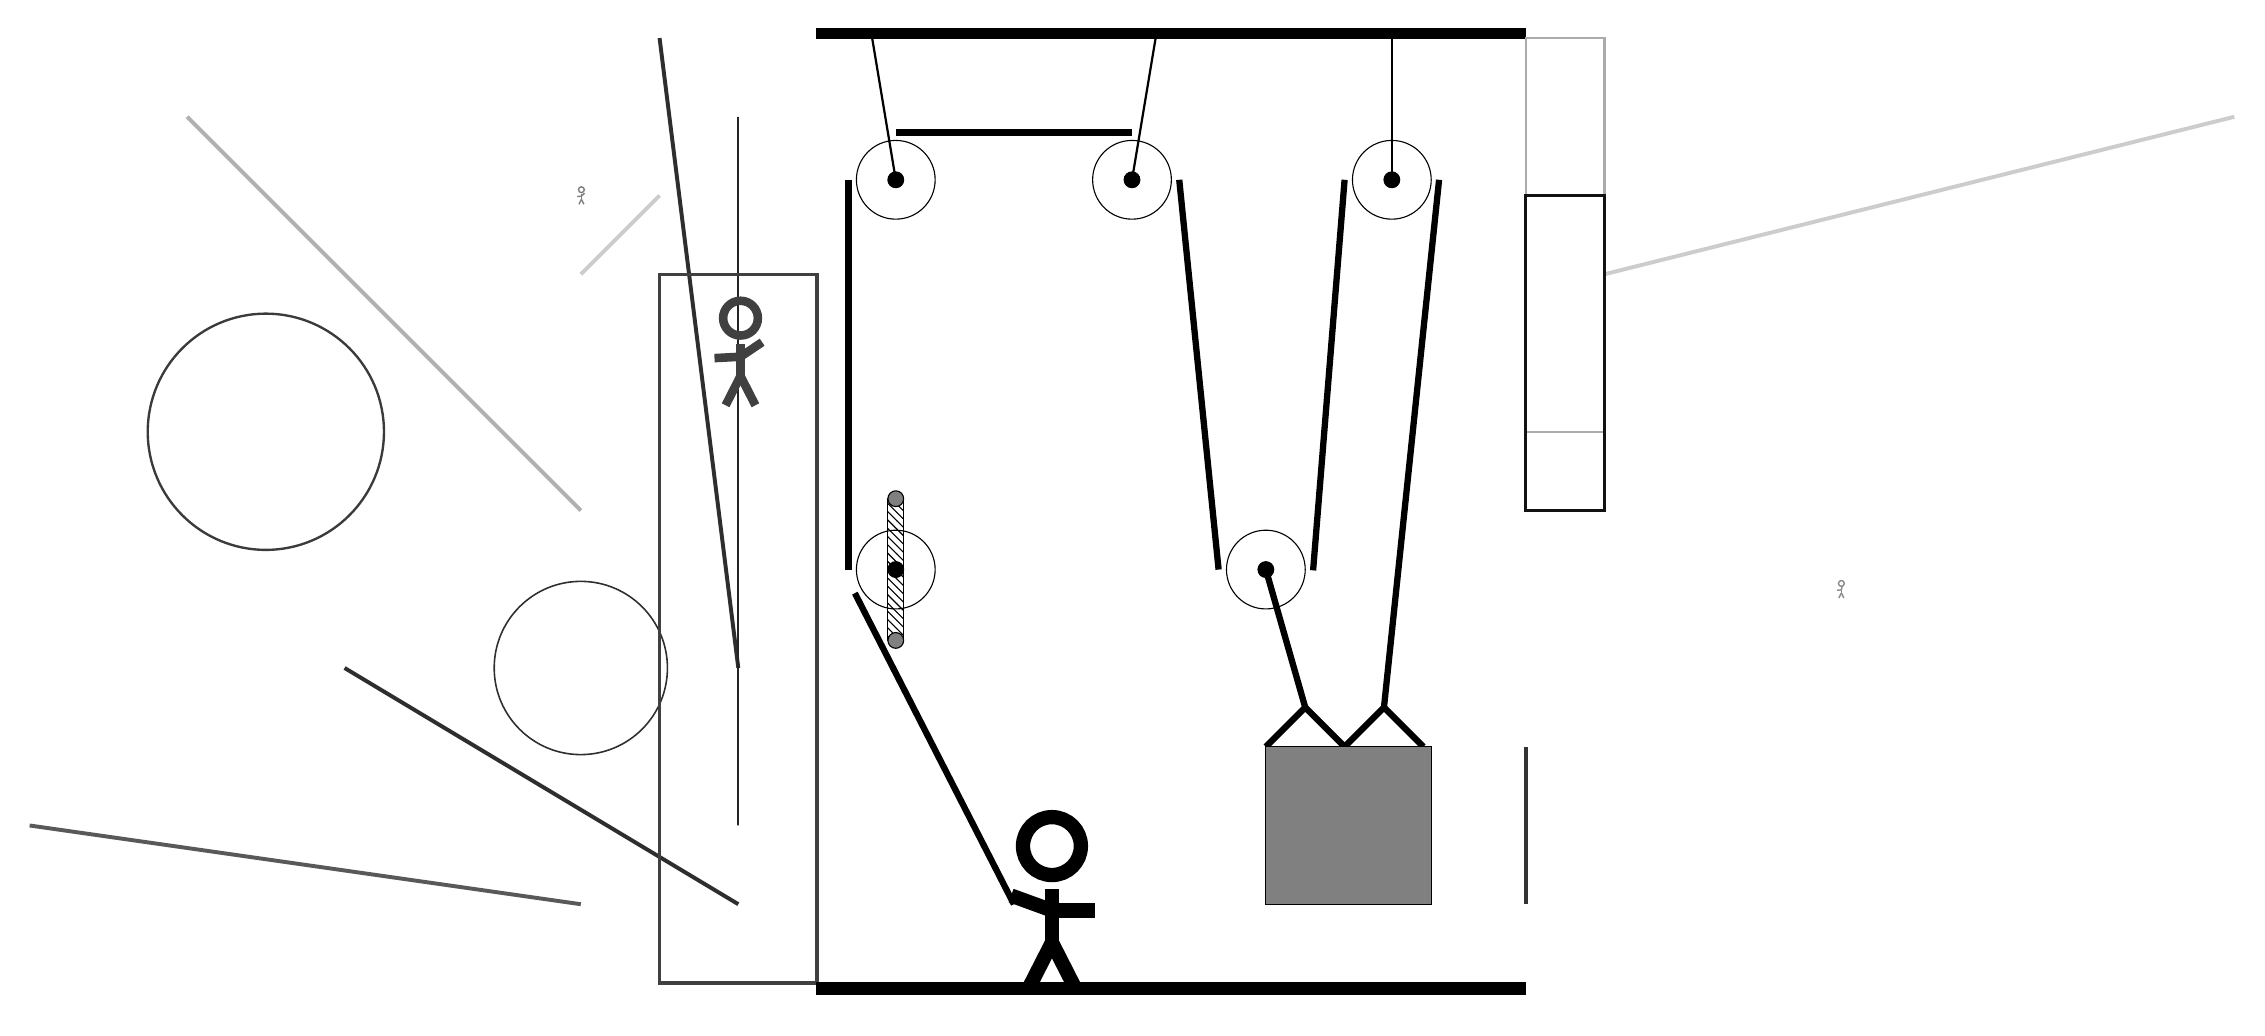
\begin{tikzpicture}
			%%%%% START %%%%%
			
			\draw[fill=black] (-3, 9) rectangle (6, 9.125);
			
			\draw (1, 7.2) circle (0.5);
			\draw[fill=black] (1, 7.2) circle (0.1);
			\draw[thick] (1, 7.2) -- (1.3, 9);
			
			\draw (4.3, 7.2) circle (0.5);
			\draw[fill=black] (4.3, 7.2) circle (0.1);
			\draw[thick] (4.3, 7.2) -- (4.3, 9);
			
			\draw (2.7, 2.25) circle (0.5);
			\draw[fill=black] (2.7, 2.25) circle (0.1);
			
			\draw[line width=0.8mm]  (2.7, 0) -- (3.2, 0.5) -- (3.7, 0) -- (4.2, 0.5) -- (4.7, 0);
			\draw[fill=black!50] (2.7, 0) rectangle (4.8, -2);
			
			\draw (-2, 7.2) circle (0.5);
			\draw[fill=black] (-2, 7.2) circle (0.1);
			\draw[thick] (-2, 7.2) -- (-2.3, 9);
			
			\draw (-2, 2.25) circle (0.5);
			\draw[fill=black] (-2, 2.25) circle (0.1);
			\draw[pattern=north west lines, pattern color=black] (-2.1, 3.15) rectangle (-1.9, 1.35);
			\draw[fill=black!50] (-2, 3.15) circle (0.1);
			\draw[fill=black!50] (-2, 1.35) circle (0.1);
			
			\draw[line width=0.8mm](-0.5, -2) -- (-2.5196, 1.95);
			\centerarc[line width=0.8mm](-2, 2.25)(180:210:0.6);
			\draw[line width=0.8mm](-2.6, 2.25) -- (-2.6, 7.2);
			\centerarc[line width=0.8mm](-2, 7.2)(90:180:0.6);
			
			\draw[line width=0.8mm](-2, 7.8) -- (1, 7.8);
			\centerarc[line width=0.8mm](1, 7.2)(0:90:0.6);
			\draw[line width=0.8mm](1.6, 7.2) -- (2.1, 2.25);
			\centerarc[line width=0.8mm](2.7, 2.25)(180:370:0.6);
			\draw[line width=0.8mm] (3.3, 2.24) -- (3.7, 7.2);
			\centerarc[line width=0.8mm](4.3, 7.2)(0:180:0.6);
			\draw[line width=0.8mm](4.2, 0.5) -- (4.9, 7.2);
			\draw[line width=0.8mm] (3.2, 0.5) -- (2.7, 2.25);
			
			\node at (0, -2) {\Strichmaxerl[10][-20][0]};
			
			\draw[line width=0.5mm, color=black!20](7, 6) -- (15, 8);
			
			\draw[line width=0.5mm, color=black!82](-4, 1) -- (-5, 9);
			\draw [line width=0.2mm, color=black!82](-6, 1) circle (1.1);
			\draw[line width=0.5mm, color=black!20](-6, 6) -- (-5, 7);
			
			\draw[line width=0.5mm, color=black!82](-4, -2) -- (-9, 1);
			
			\draw[line width=0.3mm, color=black!86] (-4, -1) rectangle (-4, 8);
			
			\draw[line width=0.5mm, color=black!65](-6, -2) -- (-13, -1);
			
			\draw[line width=0.5mm, color=black!31](-6, 3) -- (-11, 8);
			\node[line width=0.6mm, color=black!75] at (-4, 5) {\Strichmaxerl[6][3][34]};
			\draw[line width=0.4mm, color=black!75] (-3, -3) rectangle (-5, 6);
			
			\draw [line width=0.3mm, color=black!77](-10, 4) circle (1.5);
			\draw[line width=0.5mm, color=black!80](6, -2) -- (6, 0);
			\node[line width=0.7mm, color=black!45] at (10, 2) {\Strichmaxerl[1][5][79]};
			
			\node[line width=0.3mm, color=black!50] at (-6, 7) {\Strichmaxerl[1][5][43]};
			\draw[line width=0.3mm, color=black!33] (7, 4) rectangle (6, 9);
			\draw[line width=0.4mm, color=black!93] (6, 3) rectangle (7, 7);
			
			
			\draw[fill=black] (-3, -3) rectangle (6, -3.15);
			
			%%%%% END %%%%%
		\end{tikzpicture}
	\end{figure}	
\end{document}